\documentclass{beamer}
%\documentclass[handout]{beamer}

\usepackage{graphics}
\usepackage{beamerthemesplit}
\usepackage{algorithmic,algorithm}
\usepackage[xcolor=pst]{pstricks}
\usepackage[spanish]{babel}

%\usepackage{default}

%%%%%%%%%%%%%%%%%%%%%%%%%%% VERSIONES %%%%%%%%%%%%%%%%%%%%%%%%%%%%%%%%%%%
\newcommand{\version}[1]{\begin{center}{\footnotesize (Versi\'on #1)}\end{center}}
%%%%%%%%%%%%%%%%%%%%%%%%%%%%%%%%%%%%%%%%%%%%%%%%%%%%%%%%%%%%%%%%%%%%%%%%%

%%% Abreviaturas

\def\ce{curva{} el\'{\i}ptica}%
\def\ces{curvas{} el\'{\i}pticas}%
\def\Ces{Curvas{} el\'{\i}pticas}%
\def\CE{Curva{} El\'{\i}ptica}%
\def\CEs{Curvas{} El\'{\i}pticas}%
\def\cf{cuerpo finito}%
\def\cfs{cuerpos finitos}%

%%% Definiciones matem\'aticas especiales

\newcommand{\Z}{\ensuremath{\mathbb{Z}}}%			Enteros
\newcommand{\Q}{\ensuremath{\mathbb{Q}}}%			Racionales
\newcommand{\A}{\ensuremath{\mathbb{A}_{2}}}%			Plano Af\'{\i}n
\newcommand{\Proy}{\ensuremath{\mathbb{P}_{2}}}%		Plano Proyectivo
\newcommand{\K}{\ensuremath{\mathbb{K}}}%			Cuerpo en general
\newcommand{\F}{\ensuremath{\mathbb{F}}}%			Cuerpo finito en general
\newcommand{\Fp}{\ensuremath{\mathbb{F}_p}}%			Cuerpo finito de orden p (primo)
\newcommand{\EFp}{\ensuremath{E(\mathbb{F}_p)}}%		Curva el\'\{i}ptica sobre un cuerpo finito de orden p (primo)
\newcommand{\Fm}{\ensuremath{\mathbb{F}_{2^m}}}%                Cuerpo finito de caractar\'{\i}stica 2, grado m
\newcommand{\Fq}{\ensuremath{\mathbb{F}_q}}%			Idem id. q (q=p^m, p primo y m entero pos.)
\newcommand{\Zn}[1]{\ensuremath{\mathbb{Z}/#1\mathbb{Z}}}%	Anillo de los enteros mod n
\newcommand{\PaI}{\ensuremath{\mathcal{O}}}%                    Punto en el Infinito
\newcommand{\PaIe}{\ensuremath{\mathcal{O}_{E}}}%               Punto en el Infinito de la curva

%%%% ``Castellanizaci\'on'' de 'algorithmic.sty'

\renewcommand{\algorithmicrequire}{\textbf{Prerequisito:}}%
\renewcommand{\algorithmicensure}{\textbf{Postrequisito:}}%
\renewcommand{\algorithmiccomment}[1]{/* #1 */}%	
\renewcommand{\algorithmicend}{\textbf{fin}}%
\renewcommand{\algorithmicif}{\textbf{si}}%
\renewcommand{\algorithmicthen}{\textbf{entonces}}%
\renewcommand{\algorithmicelse}{\textbf{si no}}%
\renewcommand{\algorithmicfor}{\textbf{para}}%
\renewcommand{\algorithmicforall}{\textbf{para todo}}%
\renewcommand{\algorithmicdo}{\textbf{hacer}}%
\renewcommand{\algorithmicwhile}{\textbf{mientras}}%
\renewcommand{\algorithmicloop}{\textbf{bucle}}%
\renewcommand{\algorithmicrepeat}{\textbf{repetir}}%
\renewcommand{\algorithmicuntil}{\textbf{hasta}}%

\floatname{algorithm}{Algoritmo}%

%%% Teoremas y dem\'as
\theoremstyle{plain}        			% Cargar el paquete theorem.sty o amsthm.sty

\theoremstyle{definition}   			% Cargar el paquete amsthm.sty

\newtheoremstyle{saltolinea}% name   		% Sacado del 'thmtest.tex'
  {9pt}%               Space above, empty = `usual value'
  {9pt}%               Space below
  {}%                  Body font
  {}%                  Indent amount (empty = no indent, \parindent = para indent)
%  {\bfseries}%         Thm head font
  {\scshape}%          Thm head font
  {}%                  Punctuation after thm head
  {\newline}%          Space after thm head: \newline = linebreak
  {}%                  Thm head spec

\theoremstyle{saltolinea}   			% Cargar el paquete amsthm.sty
\newtheorem{algo}{Algoritmo}

\hypersetup{pdfpagemode=FullScreen}

\title[An\'alisis de ElGamal con \ces{} para el GnuPG]{An\'alisis del cifrado ElGamal de un m\'odulo con \ces{} propuesto para el GnuPG}
%\author[Sergi Blanch i Torn\'e y Ramiro Moreno Chiral]{Sergi Blanch i Torn\'e \\ sblanch@alumnes.udl.cat \\ Ramiro Moreno Chiral \\ ramiro@matematica.udl.cat}
\author[Sergi Blanch y Ramiro Moreno]{Sergi Blanch i Torn\'e \and Ramiro Moreno Chiral}
%\author[Sergi Blanch i Torn\'e]{Sergi Blanch i Torn\'e \\ sblanch@alumnes.udl.cat}
%\author[Ramiro Moreno Chiral]{Ramiro Moreno Chiral \\ ramiro@matematica.udl.cat}
\institute[Universidad de Lleida]{Criptograf\'{\i}a y Grafos\\ Departamento de Matem\'aticas\\ Universidad de Lleida}
\date{11 de septiembre de 2007}

\begin{document}


%------------------------------------ Frame 1 -----------------------------------%
%\frame{\titlepage}
\begin{frame}
  \titlepage
%  \version{2.1}
\end{frame}
%--------------------------------------------------------------------------------%


%------------------------------------ Frame 2 -----------------------------------%
\begin{frame}
\frametitle{Outline}
\tableofcontents[hideallsubsections]
\end{frame}
%--------------------------------------------------------------------------------%



%%%%%%%%%%%%%%%%%%%%%%%%%%%%%%%%%%%%%%%%%%%%%%%%%%%%%%%%%%%%%%%%%%%%%%%%%%%%%%%%%%%%%%%%%%%%%%%%%%%%
\section{Introducci\'on}
%%%%%%%%%%%%%%%%%%%%%%%%%%%%%%%%%%%%%%%%%%%%%%%%%%%%%%%%%%%%%%%%%%%%%%%%%%%%%%%%%%%%%%%%%%%%%%%%%%%%

%%%%%%%%%%%%%%%%%%%%%%%%%%%%%%%%%%%%%%%%%%%%%%%%%%%%%%%%%%%%%%%%%%%%%%%%%%%%%%%%%%%%%%%%%%%%%%%%%%%%
\subsection{El GnuPG}

%------------------------------------ Frame 3 -----------------------------------%
\begin{frame}
\frametitle{Algunas caracter\'{\i}sticas}
	%\begin{quote}\emph{Un descripci\'on breve del GnuPG. Usando 'itemize':}\end{quote}
	\pause
	  \begin{itemize}[<+-| alert@+>]
		%\item Una caracter\'{\i}stica: por ej., es \emph{Open Source}.
		\item Al decir \emph{GnuPG} uno piensa en \emph{software libre}.
		\item Software criptogr\'afico de prop\'osito general: \\cumple con est\'andares como el rfc2440.
		\item Proyecto eccGnuPG: 
		\begin{itemize}[<+-| alert@+>]
			\item GnuPG v1.4: Soporta de cifrado y firma con {\ce}.
			\item GnuPG v2: Soporta firma y tiene proyectado el cifrado.
			\item[] Filosof\'{\i}a modular de \emph{Unix}:\\Cosas peque\~nas que hacen muy bien tareas simples y que al unirlas hacen bien tareas complejas.
% 			\begin{itemize}[<+-| alert@+>]
% 				\item Basics of the Unix Philosophy
% 				\begin{itemize}[<+-| alert@+>]
% 					\item Rule of Modularity: Write simple parts connected by clean interfaces.
% 				\end{itemize}
% 			\end{itemize}
			\item {\begin{center}\framebox[8.25cm][l]{\begin{minipage}[t]{8cm}{\blue LibPth + LibGpg-error + \emph{LibGcrypt} +\\ LibAssuan + LibKsba + Gnupg-2.0}\end{minipage}}\end{center}}
		\end{itemize}
		\item Y, sobre todo, es un \emph{sistema h\'{\i}brido}.
	  \end{itemize}
\end{frame}
%--------------------------------------------------------------------------------%


%------------------------------------ Frame 4 -----------------------------------%
\begin{frame}
\frametitle{Sistemas h\'{\i}bridos}
	\pause
	\begin{figure}\begin{center}
	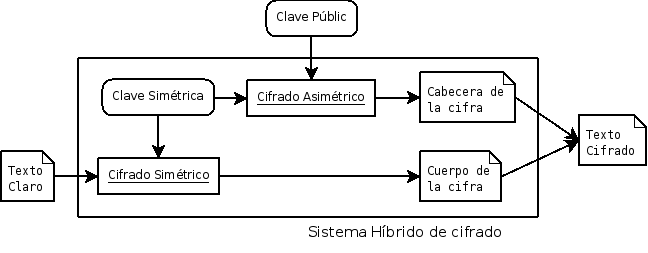
\includegraphics[scale=0.5,clip]{../imgs/sis_hibrido.png}
	\caption{Esquema de funcionamiento de un sistema h\'{\i}brido de cifrado.}\label{hibrido}
	\end{center}\end{figure}
\end{frame}
%--------------------------------------------------------------------------------%


%%%%%%%%%%%%%%%%%%%%%%%%%%%%%%%%%%%%%%%%%%%%%%%%%%%%%%%%%%%%%%%%%%%%%%%%%%%%%%%%%%%%%%%%%%%%%%%%%%%%
\subsection{\Ces}

%------------------------------------ Frame 5 -----------------------------------%
\begin{frame}
\frametitle{Nociones sobre \ces}
	\pause
	\uncover<2->{\alert<2>{Una \ce{} definida sobre un cuerpo finito est\'a determinada por una ecuaci\'on de Weierstra\ss{}
\begin{equation}\label{eq:WRF}E/\Fp:\;y^2=x^3+ax+b\text{, donde }a,b\in\Fp\text{ y } 4a^3+27b^2\ne 0.\end{equation}}}
	\uncover<3->{\alert<3>{Grupo de puntos:
$$E(\Fp)=\{(x,y)\in\Fp\times\Fp:\;y^2=x^3+ax+b\}\cup\{\mathcal{O}\}$$}}
%El conjunto $E(\Fp)$, formado por los puntos $P=(x,y)\in\Fp\times\Fp$ que satisfacen \eqref{eq:WRF} y el \emph{punto del infinito}, $\mathcal{O}$, se dota de estructura de grupo con una \emph{suma} de la que $\mathcal{O}$ es el neutro. 

%El grupo $E(\Fp)$ o es c\'{\i}clico o isomorfo a un grupo producto de dos c\'{\i}clicos.}}

	\uncover<4>{\alert<4>{Si $k$ es un entero y $P\in E(\Fp)$, escribiremos $\overbrace{P+\dots+P}^{(k}=k\cdot P$.}}
\end{frame}
%--------------------------------------------------------------------------------%


%%%%%%%%%%%%%%%%%%%%%%%%%%%%%%%%%%%%%%%%%%%%%%%%%%%%%%%%%%%%%%%%%%%%%%%%%%%%%%%%%%%%%%%%%%%%%%%%%%%%
\section{Cifrado tipo ElGamal}
%%%%%%%%%%%%%%%%%%%%%%%%%%%%%%%%%%%%%%%%%%%%%%%%%%%%%%%%%%%%%%%%%%%%%%%%%%%%%%%%%%%%%%%%%%%%%%%%%%%%

%%%%%%%%%%%%%%%%%%%%%%%%%%%%%%%%%%%%%%%%%%%%%%%%%%%%%%%%%%%%%%%%%%%%%%%%%%%%%%%%%%%%%%%%%%%%%%%%%%%%
\subsection{ElGamal en grupos c\'{\i}clicos cualesquiera}

%------------------------------------ Frame 6 -----------------------------------%
\begin{frame}
\frametitle{Cifrado ElGamal en $\mathcal{G}=\langle g\rangle$}
	\pause
\uncover<2->{Dado un grupo c\'{\i}clico cualquiera $\mathcal{G}=\langle g\rangle$, con notaci\'on multiplicativa, el cifrado ElGamal consiste en usar el intercambio de claves Diffie--Hellman (DH) como una parte de la cifra.}
	\pause
\begin{enumerate}[<+-| alert@+>]
	\item Se calcula $\alpha=g^r$, donde $1\le r<|\mathcal{G}|$ es una clave de sesi\'on aleatoria.
	\item Se convierte el mensaje $m$ en un elemento del grupo, $m\in\mathcal{G}$.
	\item En $\mathcal{G}$ se calcula $\beta=m.(g^a)^r$, siendo $k=g^a$ la clave p\'ublica del receptor. La clave com\'un DH es $k_{DH}=g^{ar}=\alpha^a$ .
	\item El mensaje cifrado es el par $(\alpha,\beta)$. 
\end{enumerate}

\uncover<7>{\alert<7>{El receptor puede recuperar el mensaje ya que $m=\beta(\alpha^a)^{-1}$ y $a$ es su clave privada.}}
\end{frame}
%--------------------------------------------------------------------------------%


%%%%%%%%%%%%%%%%%%%%%%%%%%%%%%%%%%%%%%%%%%%%%%%%%%%%%%%%%%%%%%%%%%%%%%%%%%%%%%%%%%%%%%%%%%%%%%%%%%%%
\subsection{ElGamal en el grupo multiplicativo de un cuerpo finito primo}

%------------------------------------ Frame 7 -----------------------------------%
\begin{frame}
\frametitle{ElGamal en el grupo $\Fp^*$}
	\pause
	\begin{algo}[Cifrado ElGamal]\label{alg:ElGamal}
	\parbox[b]{\linewidth}{%
	\hrule
	\smallskip
	{\bf INPUT}: Clave p\'ublica $pkey_U$ y mensaje a cifrar $m\in\Fp^*$.
	
	{\bf OUTPUT}: Cifrado formado por un par de enteros, $(\alpha,\beta)\in\Fp^*\times\Fp^*$.
	\hrule
	}%
	\begin{algorithmic}[1]
	\STATE Generar una clave de sesi\'on $r\in_{\mathcal{R}}\left[1,\left(pkey_U.p\right)-1\right]$;
	\STATE $\alpha=(pkey_U.g)^r\mod p$;
	\STATE $k_{DH}=(pkey_U.k)^r\mod p$; \\
	\COMMENT{$k=g^a\mod p$; $k_{DH}=g^{ar}\mod p$}
	\STATE $\beta=mk_{DH}\mod p$;
	\STATE Return $(\alpha,\beta)$;
	\end{algorithmic}
	\end{algo}%
\end{frame}

%--------------------------------------------------------------------------------%

%------------------------------------ Frame 8 -----------------------------------%
\begin{frame}
\frametitle{ElGamal en el grupo $\Fp^*$: comentarios}
	\pause
	\begin{itemize}[<+-| alert@+>]
		\item Pasar los mensajes al grupo es f\'acil: basta convertirlos en enteros en el rango $[1..p-1]$.
		\item Las operaciones en el grupo son productos y potencias $\mod p$, pocos pero $p$ grande.
		\item La seguridad es \emph{aproximadamente} la de un RSA cuyo m\'odulo tenga el mismo n\'umero de bits que $p$.
	\end{itemize}
\end{frame}
%--------------------------------------------------------------------------------%

%%%%%%%%%%%%%%%%%%%%%%%%%%%%%%%%%%%%%%%%%%%%%%%%%%%%%%%%%%%%%%%%%%%%%%%%%%%%%%%%%%%%%%%%%%%%%%%%%%%%
\subsection{Esquema El\'{\i}ptico ElGamal: ECElGamal}

%------------------------------------ Frame 9 -----------------------------------%
\begin{frame}
\frametitle{Esquema El\'{\i}ptico ElGamal: ECElGamal}
	\pause
	\uncover<2->{\begin{algo}[Cifrado ECElGamal]\label{alg:ECElGamal}
	\parbox[b]{\linewidth}{%
	\hrule
	\smallskip
	{\bf INPUT}: Clave p\'ublica $pkey_U$ y texto en claro num\'erico $m$.
	
	{\bf OUTPUT}: Cifrado formado por un par de puntos, $(A,B)$.
	\hrule
	}%
	\begin{algorithmic}[1]
	\STATE Generar una clave de sesi\'on $r\in_{\mathcal{R}}\left[1,\left(pkey_U.n\right)-1\right]$;
	\STATE $A=r\cdot (pkey_U.G)$;
	\STATE $K_{DH}=r\cdot (pkey_U.K)$; \COMMENT{$K=a\cdot G$; $K_{DH}=(ra)\cdot G$}
	\STATE Convertir el mensaje en punto de la \ce{} $m\rightarrow M$;
	\STATE $B=M+A$;
	\STATE Return $(A,B)$;
	\end{algorithmic}
	\end{algo}}

	\uncover<3>{\alert<3>{Se recupera $m$ calculando $M=B+a\cdot(-A)$ y, finalmente, se pasa $M\rightarrow m$.}}
\end{frame}
%--------------------------------------------------------------------------------%

%------------------------------------ Frame 10 ----------------------------------%
\begin{frame}
\frametitle{ECElGamal: comentarios}
	\pause
	\begin{itemize}[<+-| alert@+>]
		\item El criptosistema se plantea en $\langle (pkey_U.G)\rangle$, subgrupo c\'{\i}clico de $E(\Fp)$ generado por el punto $G$.
		\item La suma de puntos consiste en varios productos $\mod p$.
		\item La seguridad equivalente a un RSA con m\'odulo de 1024 bits se consigue en \ces{} sobre un cuerpo finito para valores de $p$ de $\sim$160 bits.
	\end{itemize}
	\uncover<5>{\begin{center}\framebox[8.25cm][l]{\begin{minipage}[t]{8cm}{\blue Pero los pasos de mensaje a punto de $E(\Fp)$, $m\rightarrow M$ y su inverso, son problem\'aticos en su implementaci\'on.}\end{minipage}}\end{center}}
\end{frame}
%--------------------------------------------------------------------------------%


%%%%%%%%%%%%%%%%%%%%%%%%%%%%%%%%%%%%%%%%%%%%%%%%%%%%%%%%%%%%%%%%%%%%%%%%%%%%%%%%%%%%%%%%%%%%%%%%%%%%
\section{Esquema ECDH+ElGamal}
%%%%%%%%%%%%%%%%%%%%%%%%%%%%%%%%%%%%%%%%%%%%%%%%%%%%%%%%%%%%%%%%%%%%%%%%%%%%%%%%%%%%%%%%%%%%%%%%%%%%

%------------------------------------ Frame 11 ----------------------------------%
\begin{frame}
\frametitle{Esquema ECDH+ElGamal}
	\pause
        \begin{overlayarea}{\textwidth}{6.65cm}
	\only<2-3>{\begin{algo}[Cifrado ECDH+ElGamal]\label{alg:ECDH}
	\parbox[b]{\linewidth}{%
	\hrule
	\smallskip
	{\bf INPUT}: Clave p\'ublica $pkey_U$ y texto en claro num\'erico $m$.
	
	{\bf OUTPUT}: Punto resultante $A$, cifra $\beta$.
	\hrule
	}%
	\vspace{-.5cm}
	\begin{algorithmic}[1]
	\STATE Generar una clave de sesi\'on $r\in_{\mathcal{R}}\left[1,\left(pkey_U.p\right)-1\right]$;
	\STATE $A=r\cdot (pkey_U.G)$;
	\STATE $K_{DH}=r\cdot (pkey_U.K)$; \COMMENT{$K=a\cdot G$; $K_{DH}=(ra)\cdot G$}
	\STATE $\beta=mx(K_{DH})\mod p$; \COMMENT{$x(K_{DH})$ es la abscisa de $K_{DH}$}
	\STATE Return $(A,\beta)$
	\end{algorithmic}
	\end{algo}}
	\vspace{-.5cm}
	\only<3>{\begin{center}\framebox[10.25cm][l]{\begin{minipage}[t]{10cm}{\blue !`Recuperaremos $m\mod p$ y no $m$! En un sistema h\'{\i}brido como el GnuPG, se puede perder la clave del cifrado sim\'etrico.}\end{minipage}}\end{center}}
	\only<4-5>{\begin{algo}[Cifrado ECDH+ElGamal]\label{alg:ECDH1}
	\parbox[b]{\linewidth}{%
	\hrule
	\smallskip
	{\bf INPUT}: Clave p\'ublica $pkey_U$ y texto en claro num\'erico $m$.
	
	{\bf OUTPUT}: Punto resultante $A$, cifra $\beta$.
	\hrule
	}%
	\vspace{-.5cm}
	\begin{algorithmic}[1]
	\STATE Generar una clave de sesi\'on $r\in_{\mathcal{R}}\left[1,\left(pkey_U.p\right)-1\right]$;
	\STATE $A=r\cdot (pkey_U.G)$;
	\STATE $K_{DH}=r\cdot (pkey_U.K)$; \COMMENT{$K=a\cdot G$; $K_{DH}=(ra)\cdot G$}
	\STATE $\beta=mx(K_{DH})\mod p$;{\red \!\!\!\!\!\!\!\!\!\!\!\!\!\!\!\!\!\!XXXX} \\
	\COMMENT{$x(K_{DH})$ es la abscisa de $K_{DH}$}
	\STATE Return $(A,\beta)$
	\end{algorithmic}
	\end{algo}}
	\vspace{-.5cm}
	\only<5>{\begin{center}\framebox[10.25cm][l]{\begin{minipage}[t]{10cm}{\blue Pero ahora $mx(K_{DH})$ puede ser un n\'umero demasiado peque\~no, susceptible de un ataque por factorizaci\'on.}\end{minipage}}\end{center}}
	\end{overlayarea}
\end{frame}
%--------------------------------------------------------------------------------%


%%%%%%%%%%%%%%%%%%%%%%%%%%%%%%%%%%%%%%%%%%%%%%%%%%%%%%%%%%%%%%%%%%%%%%%%%%%%%%%%%%%%%%%%%%%%%%%%%%%%
\section{Esquema alternativo ECDH+AES256}
%%%%%%%%%%%%%%%%%%%%%%%%%%%%%%%%%%%%%%%%%%%%%%%%%%%%%%%%%%%%%%%%%%%%%%%%%%%%%%%%%%%%%%%%%%%%%%%%%%%%

%------------------------------------ Frame 12 ----------------------------------%
\begin{frame}
\frametitle{Esquema alternativo ECDH+AES256}
	\pause
	\begin{algo}[Cifrado ECDH+AES]\label{alg:AES}
	\parbox[b]{\linewidth}{%
	\hrule
	\smallskip
	{\bf INPUT}: Clave p\'ublica $pkey_U$ y texto en claro num\'erico $m$.
	
	{\bf OUTPUT}: Punto resultante $A$, cifra $\beta$.
	\hrule
	}%
	\begin{algorithmic}[1]
	\STATE Generar una clave de sesi\'on $r\in_{\mathcal{R}}\left[1,\left(pkey_U.n\right)-1\right]$;
	\STATE $A=r\cdot (pkey_U.G)$;
	\STATE $K_{DH}=r\cdot (pkey_U.K)$;\\
	\COMMENT{$K=a\cdot G$; $K_{DH}=(ra)\cdot G$}
	\STATE $\beta=\textrm{aes256}(m,\{\textrm{sha256}(x(K_{DH}))\})$;\\
	\COMMENT{$x(K_{DH})$ es la abscisa de $K_{DH}$}
	\STATE Return $(A,\beta)$
	\end{algorithmic}
	\end{algo}
\end{frame}
%--------------------------------------------------------------------------------%

%------------------------------------ Frame 13 ----------------------------------%
\begin{frame}
\frametitle{ECDH + AES256: comentarios}
	%\begin{quote}\emph{Te listo algunas ideillas \dots}\end{quote}
	\pause
	\begin{itemize}[<+-| alert@+>]
		%\item Comentar el ``statement'' 4 del \emph{ECDH + AES256} para que quede claro (es muy complejo: tal vez ser\'{\i}a m\'as conveniente explicarlo directamente en la ``transpa'' anterior).
		\item ?`Qu\'e significa $\beta=\textrm{aes256}(m,\{\textrm{sha256}(x(K_{DH}))\})$?
		\begin{itemize}[<+-| alert@+>]
			\item Queremos cifrar $m$ con la clave $x(K_{DH})$ con un \emph{aes256}.
			\item La clave $x(K_{DH})$ ha de ser de tama\~no m\'aximo\\ y recuperable por el receptor: $\textrm{sha256}(x(K_{DH}))$.
		\end{itemize}
		\item Podr\'{\i}amos resumirlo como una operaci\'on: \begin{equation}
		                                                      \beta=m  \otimes  (x(K_{DH}))
		                                                     \end{equation} 
		\item La resistencia del valor $\beta$ queda garantizada por la del $\textrm{aes256}$.
	\end{itemize}
\end{frame}
%--------------------------------------------------------------------------------%


%%%%%%%%%%%%%%%%%%%%%%%%%%%%%%%%%%%%%%%%%%%%%%%%%%%%%%%%%%%%%%%%%%%%%%%%%%%%%%%%%%%%%%%%%%%%%%%%%%%%
\section{Conclusi\'on}
%%%%%%%%%%%%%%%%%%%%%%%%%%%%%%%%%%%%%%%%%%%%%%%%%%%%%%%%%%%%%%%%%%%%%%%%%%%%%%%%%%%%%%%%%%%%%%%%%%%%

%------------------------------------ Frame 14 ----------------------------------%
\begin{frame}
\frametitle{Conclusi\'on}
	%\begin{quote}\emph{Igualmente algunas ideillas \dots}\end{quote}
	\pause
	\begin{itemize}[<+-| alert@+>]
		\item Las debilidades aparecen seg\'un los contextos: el \emph{ECDH+ElGamal} $\mod p$, es un algoritmo te\'orico admitido y difundido, pero no se puede usar en el contexto h\'{\i}brido del GnuPG y, en general, cuando $m>p$.
		\item Potencia del \emph{Open Source}: Mikael Mylnikov.
		\item GnuPG v1.4 ya soporta el esquema ECDH + AES256 de forma experimental.
		\item GnuPG v2 va a implementar, nativamente desde la librer\'{\i}a \emph{LibGcrypt}, este esquema.
	\end{itemize}
\end{frame}
%--------------------------------------------------------------------------------%


\end{document}
